\documentclass[border=1mm]{standalone}
% \usepackage[margin=2.5cm]{geometry}

\usepackage{graphicx,tikz,tikz-layers} 
\usetikzlibrary{decorations.markings,calc,positioning,arrows,shapes.geometric,arrows.meta,matrix}
\usetikzlibrary{3d,perspective}


\colorlet{myred}{red!80!black}
\colorlet{myblue}{blue!80!black}
\colorlet{mybluee}{myblue!80!black}
\colorlet{mygreen}{green!60!black}
\colorlet{myorange}{orange!70!red!60!black}
\colorlet{mydarkred}{red!20!black}
\colorlet{mydarkblue}{blue!40!black}
\colorlet{mydarkgreen}{green!20!black}


\begin{document}

% \resizebox{\textwidth}{!}{
% \tikz[font=\small,scale=1, every node/.style={outer sep=0pt, inner sep=0pt, align=center, fill=white}, w/.style={minimum width=#1},h/.style={minimum height=#1},s/.style={minimum size=#1}, eu/.style={shorten >=#1},ed/.style={shorten <=#1},line join=round]
% {
% \tikzset{>={Latex[length=1.5mm, width=1.25mm]}}


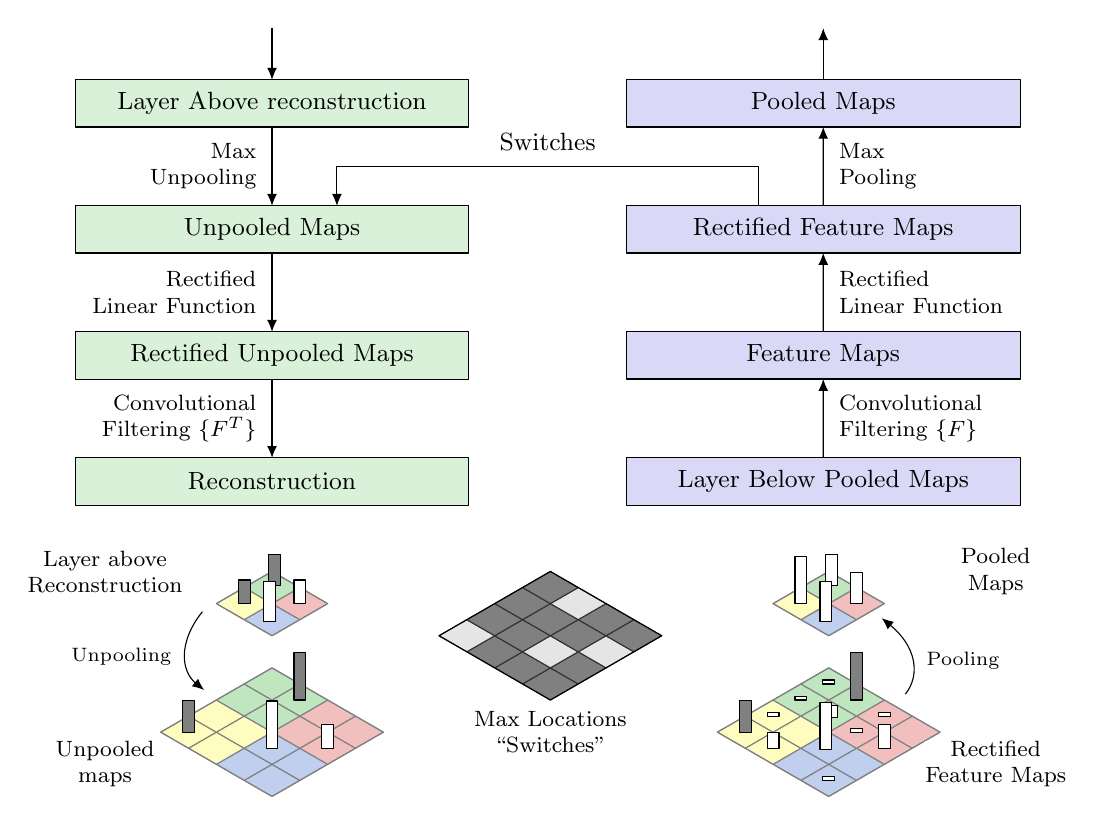
\begin{tikzpicture}[font=\small,scale=1, every node/.style={outer sep=0pt, inner sep=0pt, align=center, fill=white}, w/.style={minimum width=#1},h/.style={minimum height=#1},s/.style={minimum size=#1}, eu/.style={shorten >=#1},ed/.style={shorten <=#1},line join=round,isometric view, canvas is xy plane at z=0]

\tikzset{>={Latex[length=1.5mm, width=1.25mm]}}

  \foreach \i in {0,0.5,1,1.5} \foreach \j in {0,0.5,1,1.5} {
    \pgfmathparse{ifthenelse(\i<1 && \j>=1, "yellow!25", ifthenelse(\i>=1 && \j>=1, "mygreen!25", ifthenelse(\i<1 && \j<1, "cyan!50!blue!25", "myred!25")))}
    \fill[\pgfmathresult,draw=gray] (\i,\j) rectangle (\i+0.5,\j+0.5);
  }
  \draw[gray] (0,0,0) rectangle (2, 2,0);

% Bars
\node[draw, fill=gray, w=.15cm, h=.4cm, anchor=south] at (.25,1.75,0) {};
\node[draw, fill=white, w=.15cm, h=.6cm, anchor=south] at (.75,.75,0) {};
\node[draw, fill=white, w=.15cm, h=.3cm, anchor=south] at (1.25,.25,0) {};
\node[draw, fill=gray, w=.15cm, h=.6cm, anchor=south] at (1.75,1.25,0) {};


% 2*2 matrix
\begin{scope}[xshift=2cm, yshift=2cm]
\foreach \i in {0,0.5} 
            \foreach \j in {0,0.5} {
                \pgfmathparse{ifthenelse(\i==0 && \j==0.5, "yellow!25", 
                               ifthenelse(\i==0.5 && \j==0.5, "mygreen!25", 
                               ifthenelse(\i==0 && \j==0, "cyan!50!blue!25", 
                               "myred!25")))}
                % Center the smaller grid above the larger one
                \fill[\pgfmathresult,draw=gray] (\i+0.5,\j+0.5,1) rectangle (\i+1,\j+1,1);
            }
        \draw[gray] (0.5,0.5,1) rectangle (1.5,1.5,1);

% Bars
\node[draw, fill=gray, w=.15cm, h=.4cm, anchor=south] at (0.5+.8,0.5+.75,0) {};
\node[draw, fill=white, w=.15cm, h=.5cm, anchor=south] at (0.5+.2,0.5+.25,0) {};
\node[draw, fill=white, w=.15cm, h=.3cm, anchor=south] at (0.5+.75,0.5+.25,0) {};
\node[draw, fill=gray, w=.15cm, h=.3cm, anchor=south] at (0.5+.25,0.5+.75,0) {};
\end{scope}

%---------------------------------------

\begin{scope}[xshift=5cm, yshift=-5cm]
  \foreach \i in {0,0.5,1,1.5} \foreach \j in {0,0.5,1,1.5} {
    \pgfmathparse{ifthenelse(\i<1 && \j>=1, "yellow!25", ifthenelse(\i>=1 && \j>=1, "mygreen!25", ifthenelse(\i<1 && \j<1, "cyan!50!blue!25", "myred!25")))}
    \fill[\pgfmathresult,draw=gray] (\i,\j) rectangle (\i+0.5,\j+0.5);
  }
  \draw[gray] (0,0,0) rectangle (2, 2,0);

% Bars
\node[draw, fill=white, w=.15cm, h=.05cm, anchor=south] at (0.25,0.25,0) {};
\node[draw, fill=white, w=.15cm, h=.05cm, anchor=south] at (1.25,0.75,0) {};
\node[draw, fill=white, w=.15cm, h=.05cm, anchor=south] at (1.75,0.75,0) {};
\node[draw, fill=white, w=.15cm, h=.15cm, anchor=south] at (1.25,1.2,0) {};
\node[draw, fill=white, w=.15cm, h=.05cm, anchor=south] at (1.25,1.75,0) {};
\node[draw, fill=white, w=.15cm, h=.05cm, anchor=south] at (1.75,1.75,0) {};
\node[draw, fill=white, w=.15cm, h=.05cm, anchor=south] at (.75,1.75,0) {};
\node[draw, fill=white, w=.15cm, h=.2cm, anchor=south] at (.25,1.25,0) {};

\node[draw, fill=gray, w=.15cm, h=.4cm, anchor=south] at (.25,1.75,0) {};
\node[draw, fill=white, w=.15cm, h=.6cm, anchor=south] at (.7,.75,0) {};
\node[draw, fill=white, w=.15cm, h=.3cm, anchor=south] at (1.25,.25,0) {};
\node[draw, fill=gray, w=.15cm, h=.6cm, anchor=south] at (1.75,1.25,0) {};
% 2*2 matrix
\begin{scope}[xshift=2cm, yshift=2cm]
\foreach \i in {0,0.5} 
            \foreach \j in {0,0.5} {
                \pgfmathparse{ifthenelse(\i==0 && \j==0.5, "yellow!25", 
                               ifthenelse(\i==0.5 && \j==0.5, "mygreen!25", 
                               ifthenelse(\i==0 && \j==0, "cyan!50!blue!25", 
                               "myred!25")))}
                % Center the smaller grid above the larger one
                \fill[\pgfmathresult,draw=gray] (\i+0.5,\j+0.5,1) rectangle (\i+1,\j+1,1);
            }
        \draw[gray] (0.5,0.5,1) rectangle (1.5,1.5,1);

% Bars
\node[draw, fill=white, w=.15cm, h=.4cm, anchor=south] at (0.5+.8,0.5+.75,0) {};
\node[draw, fill=white, w=.15cm, h=.5cm, anchor=south] at (0.5+.2,0.5+.25,0) {};
\node[draw, fill=white, w=.15cm, h=.4cm, anchor=south] at (0.5+.75,0.5+.25,0) {};
\node[draw, fill=white, w=.15cm, h=.6cm, anchor=south] at (0.5+.25,0.5+.75,0) {};
\end{scope}
\end{scope}

\begin{scope}[xshift=4cm, yshift=-1cm]
\foreach \i in {0,0.5,1,1.5} 
  \foreach \j in {0,0.5,1,1.5} {
    \pgfmathparse{ifthenelse(
      (\i==0 && \j==1.5) || (\i==1 && \j==0) || (\i==0.5 && \j==.5) || (\i==1.5 && \j==1),
      "gray!20", "gray"
    )}
    \fill[\pgfmathresult,draw=black!80] (\i,\j) rectangle (\i+0.5,\j+0.5);
}
\draw[] (0,0) rectangle (2,2);
\end{scope}

\node[font=\footnotesize] at (-1,2) {Unpooled\\maps};
\node[font=\footnotesize] at (2,5) {Layer above\\Reconstruction};

\node[font=\footnotesize] at (7,-6) {Rectified\\Feature Maps};
\node[font=\footnotesize] at (10,-3) {Pooled\\Maps};

\node[font=\footnotesize] at (3.5,-1.5) {Max Locations\\``Switches''};

\draw[<-, ed=2mm] (1,2) to[bend left] node[left=2mm] {\scriptsize Unpooling} +(1.25,1.5);
\draw[->, ed=2mm] (7,-4.2) to[bend right] node[right=2mm] {\scriptsize Pooling} +(1.25,1.5);

%------------------------
\node[draw, w=5cm, h=.6cm, yshift=4cm, fill=mygreen!15] (a) {Reconstruction};
\node[draw, w=5cm, h=.6cm, right=2cm of a, fill=myblue!15] (b) {Layer Below Pooled Maps};
\node[draw, w=5cm, h=.6cm, above=1cm of a, fill=mygreen!15] (c) {Rectified Unpooled Maps};
\node[draw, w=5cm, h=.6cm, right=2cm of c, fill=myblue!15] (d) {Feature Maps};
\node[draw, w=5cm, h=.6cm, above=1cm of c, fill=mygreen!15] (e) {Unpooled Maps};
\node[draw, w=5cm, h=.6cm, right=2cm of e, fill=myblue!15] (f) {Rectified Feature Maps};
\node[draw, w=5cm, h=.6cm, above=1cm of e, fill=mygreen!15] (g) {Layer Above reconstruction};
\node[draw, w=5cm, h=.6cm, right=2cm of g, fill=myblue!15] (h) {Pooled Maps};

\draw[->] (b)--node[align=left, right=2mm, font=\footnotesize] {Convolutional\\Filtering $\{F\}$} (d);
\draw[->] (d)--node[align=left, right=2mm, font=\footnotesize] {Rectified\\Linear Function} (f);
\draw[->] (f)--node[align=left, right=2mm, font=\footnotesize] {Max\\Pooling} (h);

\draw[<-] (a)--node[align=right, left=2mm, font=\footnotesize] {Convolutional\\Filtering $\{F^T\}$} (c);
\draw[<-] (c)--node[align=right, left=2mm, font=\footnotesize] {Rectified\\Linear Function} (e);
\draw[<-] (e)--node[align=right, left=2mm, font=\footnotesize] {Max\\Unpooling} (g);

\draw[<-] (g.north) -- +(0.8,0.8);
\draw[->] (h.north) -- +(0.8,0.8);

\begin{scope}[reset cm]
\draw[->] (f.160)--++(0,.5) -| node[above=2mm, pos=.25] {Switches} (e.20);
\end{scope}

\end{tikzpicture}



% }
% }
\end{document}
